\documentclass[12pt]{article}%

\usepackage{fancyhdr}
\pagestyle{fancy}
\fancyhf{}
\fancyhead[R]{\thepage}

\usepackage{cmap}				
\usepackage{mathtext} 
\usepackage{listings}

\usepackage{biblatex}
\addbibresource{lib.bib}

\usepackage{euscript}
\usepackage{mathrsfs}

\usepackage[T2A]{fontenc}
\usepackage[utf8]{inputenc}
\usepackage[english,russian]{babel}
\usepackage{amsmath,amsfonts,amssymb,amsthm,mathtools}

\setlength\fboxsep{3pt}
\setlength\fboxrule{1pt}

% Работа с графикой и рисунками
\usepackage{graphicx} 
\usepackage{subcaption}

\usepackage{hyperref}
\usepackage[usenames,dvipsnames,svgnames,table,rgb]{xcolor}
\usepackage{wrapfig}
\hypersetup{				
    unicode=true,           
    pdftitle={Заголовок},   
    pdfsubject={Тема},      
    pdfkeywords={keyword1} {key2} {key3},
    colorlinks=true,
    linkcolor=black,
    citecolor=black,
    filecolor=magenta,
    urlcolor=cyan
}

% Работа с Python
\usepackage{minted}
\definecolor{LightGray}{gray}{0.98}

% Работа с enumerate
\usepackage{enumitem}

\newcommand*{\Title}{\begingroup
\centering 

\large {Федеральное автономное образовательное учреждение высшего образования}
\vspace*{\baselineskip}

\large {«Национальный исследовательский университет «Высшая школа экономики»»}
\vspace*{\baselineskip}

\vspace*{\baselineskip}
\large{\textbf{Отчет по лабораторной работе 6}}

\vspace{0.1cm}
\large{Численное решение задачи Коши}

\vspace{0.2cm}
\large{Вариант 10: задачи 7.1.10, 7.3.4, 7.5.4}

\vspace{1.5cm} 

\begin{flushright}
  \textbf{\normalsize Выполнил:}
  
  \vspace{0.3cm} 
  {\normalsize Студент группы БПМ-211}
  
  {\normalsize Ляхов Артём Андреевич}

\end{flushright}


\vspace{0.2cm}  
\begin{flushright}
  \textbf{\normalsize Преподаватель:} 

  \vspace{0.2cm}

 {\normalsize Брандышев Петр Евгеньевич}
 
\end{flushright}

\vfill
\date{}{Июнь 2024 г.}


\endgroup\clearpage}

\begin{document}
\Title
\tableofcontents

\newpage
\section{Задача 7.1.10. Метод Эйлера и метод Рунге-Кутты 4 порядка для решения задачи Коши}
\subsection{Формулировка задачи}
Необходимо найти приближённое решение задачи Коши для ОДУ первого порядка:
$$
\begin{cases}
    y'(t) = f(t, y(t)) \\
    y(t_0) = y_0
\end{cases}
$$
на отрезке $t \in [t_0, T]$. 

Решение задачи должно состоять из следующих шагов:
\begin{enumerate}
    \item Задать исходные данные $f(t, y)$, $y_0$ $t_0$, $T$.
    \item Написать функцию, реализующую метод Эйлера, и с её помощью найти приближенное решение задачи Коши с шагом $h=0.1$.
    \item Написать функцию, реализующую метод Рунге-Кутты четвёртого порядка, и с её помощью найти решение задачи Коши с шагом $h=0.1$.
    \item Найти решение задачи Коши аналитически.
    \item На одном рисунке построить графики приближённых и точного решений.
    \item Оценить погрешность найденных решений двумя различными способами:
    \begin{itemize}
        \item по формуле $\varepsilon = \max\limits_{0 \leqslant i \leqslant N}|y(t_i) - y_i|$, где $y(t)$ - аналитическое решение, $y_i$ - значение приближённого значения в узле сетки.
        \item по правилу Рунге (по правилу двойного пересчёта).
    \end{itemize}
    \item Выяснить при каком значении шага $h = h^*$ решение, полученное по методу Эйлера, будет иметь такую же погрешность, как решение, полученное с помощью метода Рунге-Кутты с шагом $h=0.1$.
\end{enumerate}

Согласно условию варианта:
$$
f(t, y) = -\frac{2t}{1 + t^2} \cdot y + \frac{2t^2}{1 + t^2},\ \ \ \ \ t_0 = 0,\ \ \ T = 1,\ \ \ y_0 = 2/3
$$

\subsection{Теоретический материал}
\subsubsection{Аналитическое решение задачи Коши}
Решаемое нами уравнение
\begin{equation}
y' = -\frac{2t}{1 + t^2}\cdot y + \frac{2 t^2}{1 + t^2}
\end{equation}
является линейным неоднородным уравнением первого порядка. Уравнения данного типа можно решать с помощью метода вариации постоянной.

Для этого сначала найдём решение соответствующего однородного уравнения. Это решение будем иметь вид:
\begin{equation}
    y(t) = \frac{C}{1 + t^2},\ \ \ C \in \mathbb{R}
\end{equation}

Затем варьируем константу, то есть представляем решение исходного уравнения в виде:
$$
y(t) = \frac{C(t)}{1 + t^2}
$$
После подстановки выражения выше в исходное уравнение получаем, что
$$
C(t) = \frac{2}{3}t^3 + E, \ \ \ E \in \mathbb{R}
$$
Используя начальное условие $y(0) = 2/3$, мы можем найти $E$ и вместе с тем выписать итоговое решение задачи Коши:
\begin{equation}
    y(t) = \frac{2}{3} \left( \frac{1 + t^3}{1 + t^2} \right)
\end{equation}

\subsubsection{Метод Эйлера}
Метод Эйлера - простейший численный метод решения обыкновенных дифференциальных уравнений.

Пусть дана задача Коши для уравнения первого порядка:
$$
\begin{cases}
    \frac{dy}{dt} = f(t, y) \\
    y |_{t = t_0} = y_0
\end{cases}
$$
Тогда согласно методу Эйлера приближённое решение в узлах $x_i$, которое мы обозначим за $y_i$, определяется через соотношение
\begin{equation}\label{euler1}
    y_i = y_{i-1} + (t_{i} - t_{i-1}) \cdot f(t_{i - 1}, y_{i - 1})
\end{equation}

Если длина шага постоянна и равна $h$, то соотношение \ref{euler1} можно переписать в виде:
\begin{equation}
    y_i = y_{i-1} + h \cdot f(t_{i-1}, y_{i - 1})
\end{equation}

Метод Эйлера является методом первого порядка и погрешность на шаге $O(h^2)$ $h \rightarrow 0$.

\subsubsection{Метод Рунге-Кутты четвёртого порядка}
Рассмотрим задачу Коши для ОДУ первого порядка:
$$
\begin{cases}
    \frac{dy}{dt} = f(t, y) \\
    y |_{t = t_0} = y_0
\end{cases}
$$
Тогда приближённое значение в последующих точках, согласно методу Рунге-Кутты 4 порядка, вычисляется по итерационной формуле:
\begin{equation}
    y_{i} = y_{i - 1} + \frac{h}{6}(k_1 + 2k_2 + 2k_3 + k_4)
\end{equation}
Вычисление нового значения производится в 4 стадии:
\begin{equation}
\begin{cases}
    k_1 = f(x_{i-1},\ y_{i-1}) \\
    k_2 = f\left(t_{i-1} + \frac{h}{2},\ y_{i-1} + \frac{h}{2}k_1 \right)\\
    k_3 = f\left(t_{i-1} + \frac{h}{2},\ y_{i-1} + \frac{h}{2}k_2 \right)\\
    k_4 = f\left(t_{i-1} + h,\ y_{i-1} + hk_3 \right)
\end{cases}
\end{equation}
где $h$ - величина шага по сетке.

Данный метод является методом четвёртого порядка, что означает, что ошибка на одном шаге имеет порядок $O(h^5)$ $h \rightarrow 0$.

\subsection{Правило Рунге}
Предположим, что $p$ - порядок метода, с помощью которого мы находим приближённое решение задачи Коши, $\hat{y}_{i}$ - приближённое решение задачи Коши в узле $t_i$, найденное при шаге $h/2$. Тогда \textit{правило Рунге} практической оценки погрешности состоит в том, чтобы использовать оценку
\begin{equation}
    y(t_i) - \hat{y_i} \approx \varepsilon_i, \ \ \  \varepsilon_i = \frac{\hat{y}_{i} - y_i}{2^p - 1}
\end{equation}

Соответственно в качестве значения итоговой погрешности мы можем использовать величину:
\begin{equation}
    \varepsilon = \max\limits_{0 \le i \le N}
    \left|\frac{\hat{y}_{i} - y_i}{2^p - 1}\right|
\end{equation}


\subsection{Результаты}
\begin{figure}[h]
    \centering
    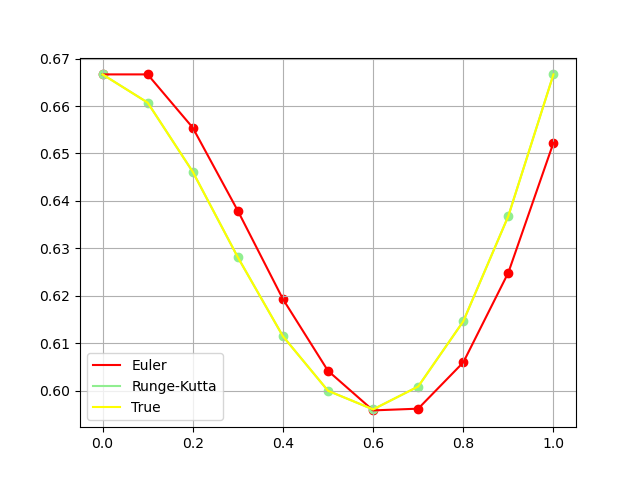
\includegraphics[width=0.8\textwidth]{task1_plots.png}
    \caption{Графики точного и приближённых решений, полученных с помощью метода Эйлера и Рунге-Кутты 4 порядка, на отрезке $[0, 1]$ с шагом сетки $h=0.1$.}
\end{figure}

\begin{table}[!h]
    \centering
    \begin{tabular}{|c|c|c|}
    \hline Метод решения & 
            $\max\limits_{0 \leqslant i \leqslant N}|y(x_i) - y_i|$ & 
            По правилу Рунге  \\
    \hline Эйлера & 
            $1.4 \cdot 10^{-2}$ & 
            $7.1 \cdot 10^{-3}$ \\
    \hline Рунге-Кутты 4 порядка & 
            $4.34 \cdot 10^{-7}$ & 
            $2.71 \cdot 10^{-8}$ \\
    \hline
    \end{tabular}
    \caption{Оценки погрешностей найденных решений задачи Коши.}
\end{table}

\newpage
\begin{table}[!h]
    \centering
    \begin{tabular}{|c|c|}
    \hline $h$ & $\max\limits_{0 \leqslant i \leqslant N}|y(x_i) - y_i|$\\
    \hline $3.05 \cdot 10^{-6}$ & $4.46 \cdot 10^{-7}$ \\
    \hline $1.52 \cdot 10^{-6}$ & $2.23 \cdot 10^{-7}$ \\
    \hline
    \end{tabular}
    \caption{Погрешность приближённых решений задачи Коши, найденных с помощью метода Эйлера, при различных значениях $h$.}
\end{table}

Таким образом, при $h = 1.52 \cdot 10^{-6}$, решение найденное с помощью метода Эйлера, имеет такую погрешность что и решение, найденное с помощью метода Рунге-Кутты 4 порядка, при $h = 0.1$.


\subsection{Код на Python}
\begin{minted}[
frame=single,
framesep=10pt,
framerule=0.1pt,
bgcolor=LightGray
]{python}
def euler(t_arr, y0, f):
    y_arr = np.zeros(t_arr.size)
    y_arr[0] = y0

    for i, t in enumerate(t_arr[1:], start=1):
        t_prev = t_arr[i - 1]
        y_prev = y_arr[i - 1]
        h = (t - t_prev)
        
        y_arr[i] = y_prev + h * f(t_prev, y_prev)

    return y_arr
\end{minted}

\begin{minted}[
frame=single,
framesep=10pt,
framerule=0.1pt,
bgcolor=LightGray
]{python}
def rkfixed(t_arr, y0, f):
    y_arr = np.zeros(t_arr.size)
    y_arr[0] = y0

    for i, t in enumerate(t_arr[1:], start=1):
        t_prev = t_arr[i - 1]
        y_prev = y_arr[i - 1]
        h = (t - t_prev)

        k1 = f(t_prev, y_prev)
        k2 = f(t_prev + h/2, y_prev + h/2 * k1)
        k3 = f(t_prev + h/2, y_prev + h/2 * k2)
        k4 = f(t_prev + h, y_prev + h * k3)

        y_arr[i] = y_prev + h/6 * (k1 + 2 * k2 + 2 * k3 + k4)

    return y_arr
\end{minted}

\newpage
\section{Задача 7.3.4 Метод Рунге-Кутты 4 порядка и экстраполяционный метод Адамса 3 порядка для решения задачи Коши}
\subsection{Формулировка задачи}
Необходимо приближённо решить задачу Коши для ОДУ первого порядка
$$
\begin{cases}
    y'(t) = f(t, y(t)) \\
    y(t_0) = y_0
\end{cases}
$$
при помощи метода Рунге-Кутты 4 порядка и метода, указанного в варианте, с шагами $h$, $h/2$. Для каждого метода необходимо оценить погрешность по правилу Рунге и вычислить уточнённое решение. Построить на одном чертеже графики приближённых решений (с шагом $h/2$) и графики уточнённых решений.

Согласно условию варианта вторым методом решения является экстраполяционный метод Адамса 3 порядка и при этом
$$
f(t, y) = y + 2ty^2 ,\ \ \ \ \ t_0 = 0,\ \ \ T = 0.8,\ \ \ y_0 = 0.5
$$

\subsection{Теоретический материал}
\subsubsection{Экстраполяционный метод Адамса 3 порядка}
Предположим, что мы хотим численно решить задачу Коши
$$
\begin{cases}
    \frac{dy}{dt} = f(t, y) \\
    y |_{t = t_0} = y_0
\end{cases}
$$
Пусть $h$ - шаг сетки, тогда приближённые значения решения в узлах сетки $y_i$, согласно экстраполяционному методу Адамса 3 порядка, вычисляются через соотношение
\begin{equation}
    y_i = y_{i-1} + \frac{h}{12}
    \left(
    23 f(t_{i-1}, y_{i-1}) - 16 f(t_{i-2}, y_{i-2}) + 5 f(t_{i-3}, y_{i-3})
    \right)
\end{equation}

\subsubsection{Правило Рунге для уточнения решения}
Правило Рунге практической оценки погрешности (правило двойного пересчёта):
$$
y(t_i) - \hat{y}_i \approx \varepsilon_{i}, \ \ \ \varepsilon_i = \frac{\hat{y}_{i} - y_i}{2^p - 1}
$$
где $y(t)$ - точное решение, $p$ - порядок метода.

Используя оценку погрешности найденного решения в узле $t_i$, мы можем построить \textit{приближённое решение}:
\begin{equation}
    y^*_i = \hat{y}_i + \varepsilon_i
\end{equation}

\subsection{Результаты}

\begin{figure}[!h]
\centering
\begin{subfigure}{0.49\textwidth}
    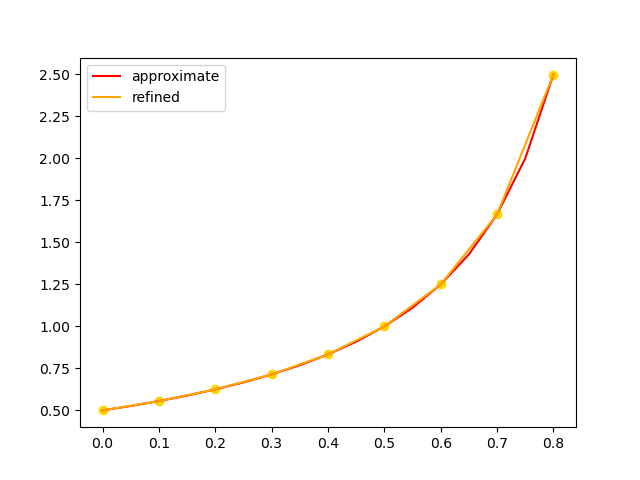
\includegraphics[width=\textwidth]{task2_rk.png}
    \caption{Метод Рунге-Кутты}
\end{subfigure}
\hfill
\begin{subfigure}{0.49\textwidth}
    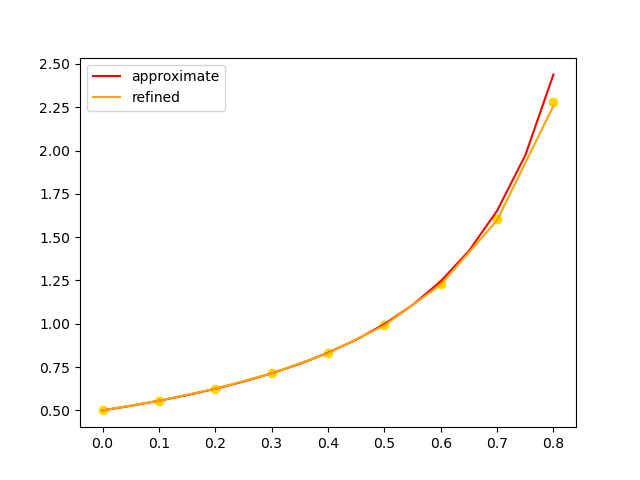
\includegraphics[width=\textwidth]{task2_adams.png}
    \caption{Метод Адамса 3 порядка}
\end{subfigure}

\caption{Визуализация приближённых и уточнённых решений задачи Коши.}
\end{figure}



\begin{table}[!h]
    \centering
    \begin{tabular}{|c|c|}
    \hline Метод & Погрешность \\
    \hline Рунге-Кутты 4 порядка & $5.09 \cdot 10^{-5}$ \\
    \hline Адамса 3 порядка & $2.2 \cdot 10^{-2}$ \\
    \hline
    \end{tabular}
    \caption{Оценки погрешностей приближённых решений по правилу Рунге.}
\end{table}

\subsection{Код на Python}
\begin{minted}[
frame=single,
framesep=10pt,
framerule=0.1pt,
bgcolor=LightGray
]{python}
def adams(t_arr, y0, f):
    h = t_arr[1] - t_arr[0]

    y_arr = np.zeros(t_arr.size)
    y_arr[0:3] = rkfixed(t_arr[0:3], y0, f)
    
    for i, t in enumerate(t_arr[3:], start=3):
        t_prev3 = t_arr[i - 3]
        y_prev3 = y_arr[i - 3]
        y3 = f(t_prev3, y_prev3)

        t_prev2 = t_arr[i - 2]
        y_prev2 = y_arr[i - 2]
        y2 = f(t_prev2, y_prev2)

        t_prev1 = t_arr[i - 1]
        y_prev1 = y_arr[i - 1]
        y1 = f(t_prev1, y_prev1)

        y_arr[i] = y_arr[i - 1] + (h/12) * \
                (23 * y1 - 16 * y2 + 5 * y3)

    return y_arr
\end{minted}

\newpage
\section{Задача 7.5.4. Сравнение метода Эйлера и метода Рунге-Кутты 4 порядка}
\subsection{Формулировка задачи}
Дана жёсткая задача Коши. Необходимо найти решение задачи с точностью $\varepsilon = 10^{-3}$.
Решение задачи должно состоять из следующих шагов:
\begin{enumerate}
    \item Используя функцию \textbf{euler}, написанную для задачи 7.1, найти приближённое решение задачи Коши явным методом Эйлера с шагом $h=0.15$. 
    \item Найти решение задачи методом Рунге-Кутты 4 порядка с помощью функции \textbf{rkfixed}, написанной для задачи 7.1 с шагом $h=0.15$.
    \item Построить графики приближённых и точного решений задачи.
    \item Уменьшая шаг, найти решения задачи с заданной точностью $\varepsilon$ каждым из методов. Сравнить значения шагов, при которых достигается точность $\varepsilon$.
    \item Объяснить полученные результаты.
\end{enumerate}
Согласно условию варианта:
$$
f(t, y) = -20y + 20 - 19 e^{-t}, \ \ \ t_0 = 0,\ T=1.5,\ y_0=1
$$
Решением задачи Коши является функция
$$
y(t) = 1 - e^{-t} + e^{-20t}
$$

\subsection{Теоретический материал}
Рассмотрим задачу Коши для системы линейных дифференциальных уравнений
\begin{equation}\label{a_system}
\begin{cases}
    u' = A(t) \cdot u(t) \\
    u(t_0) = u_0
\end{cases}
\end{equation}
где $u = u(t)$ - вектор функция, $A(t)$ - матрица-функция.

Будем называть систему выше жёсткой если, если число жёсткости системы
\begin{equation}
    S = \frac{
    \max\limits_{1 \leqslant i \leqslant n}|\lambda_i|}{
    \min\limits_{1 \leqslant i \leqslant n}|\lambda_i|}
\end{equation}
достаточно велико.


Любое линейное неоднородное уравнение первого порядка вида:
$$
y'(t) = a_1 y(t) + f(t)
$$
можно представить в виде \ref{a_system}, для этого достаточно ввести новую функцию $u(t) = f(t)$. Исходя из этого, мы будем говорить, что задачи Коши для ЛНУ первого порядка является жёсткой, если является жёсткой соответствующая ей система \ref{a_system}.

Для жёстких систем характерно то, что для них явные методы численного решения (метод Эйлера, методы Рунге-Кутты, методы Адамса и др.), как правило, показывают неудовлетворительные результаты, что выражается в резком увелечении числа итераций или резком возрастании погрешности (взрыв погрешности). В то же время неявные методы для данного класса задач показывают результаты лучше, чем явные.



\subsection{Результаты}
\begin{figure}[!h]
\centering
\begin{subfigure}{0.49\textwidth}
    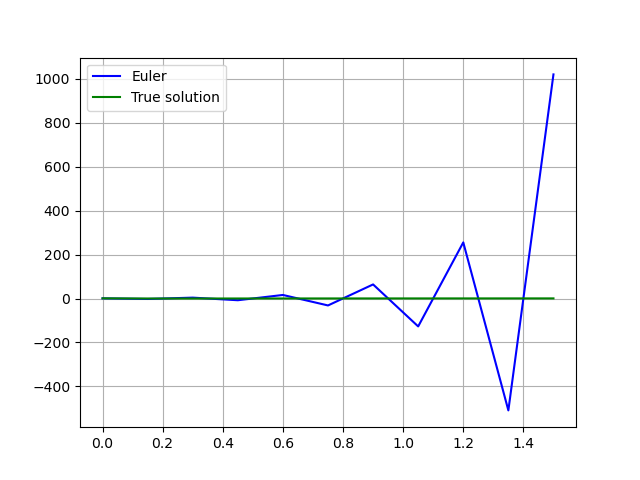
\includegraphics[width=\textwidth]{task3_euler.png}
    \caption{Метод Эйлера}
\end{subfigure}
\hfill
\begin{subfigure}{0.49\textwidth}
    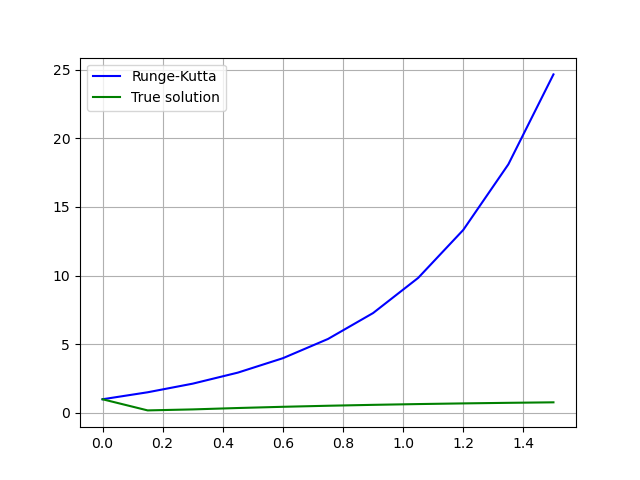
\includegraphics[width=\textwidth]{task3_rk.png}
    \caption{Метод Рунге-Кутты 4 порядка}
\end{subfigure}

\caption{Визуализация приближённых решений, найденных при помощи метода Эйлера и метода Рунге-Кутты 4 порядка, при $h = 0.15$.}
\end{figure}

\newpage
\begin{table}[!h]
    \centering
    \begin{tabular}{|c|c|c|}
    \hline Метод решения & Длина шага $h$ & Погрешность \\
    \hline Эйлера & $1.4 \cdot 10^{-4}$ & $5.4 \cdot 10^{-4}$ \\
    \hline Рунге-Кутты & $2.9 \cdot 10^{-2}$ & $5.7 \cdot 10^{-4}$ \\
    \hline
    \end{tabular}
    \caption{Длины шагов сетки, при которых достигается точность $\varepsilon = 10^{-3}$. В качестве погрешности бралась величина $\max\limits|y(x_i) - y_i|$.}
\end{table}

\textbf{Вывод:} Анализируя графики, мы можем сделать два наблюдения.
Во-первых, при длине шага $h=0.15$ приближённые решения системы, найденные с помощью метода Эйлера и Рунге-Кутты, имеют огромную погрешность. Во-вторых, для того, чтобы достичь требуемой точности решения в $10^{-3}$, нам необходимо сделать шаг по сетке достаточно маленьким, что говорит о неэффективности метода Эйлера и метода Рунге-Кутты 4 порядка для данной задачи. Оба этих факта легко объясняются тем, что решаемая задача Коши является жёсткой.


\end{document}